\documentclass[border=2pt]{standalone}

\usepackage{tikz}
\tikzset{>=latex}

\begin{document}
	
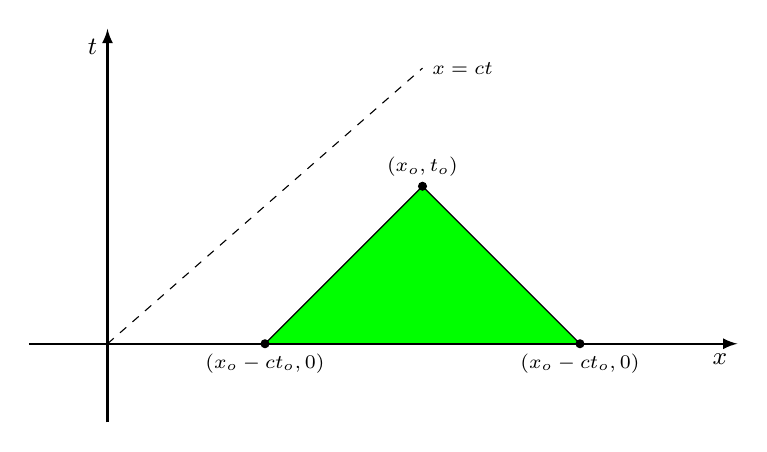
\begin{tikzpicture}
	\path [fill=green] (4,2) -- (2,0) -- (6,0) -- (4,2);
	\draw [->, thick] (-1,0) -- (8,0) node [below left] {\small$x$};
	\draw [->, thick] (0,-1) -- (0,4)  node [below left] {\small$t$};
	\draw (2,0) -- (4,2);
	\draw (4,2) -- (6,0);
	\draw [dashed] (0,0) -- (4,3.5) node [right] {\scriptsize$x=ct$};
	\draw [fill] (4,2) circle [radius=.05] node [above] {\scriptsize$(x_{o},t_{o})$};
	\draw [fill] (6,0) circle [radius=.05] node [below] {\scriptsize$(x_{o}-ct_{o},0)$};	
	\draw [fill] (2,0) circle [radius=.05] node [below] {\scriptsize$(x_{o}-ct_{o},0)$};
\end{tikzpicture}

\quad

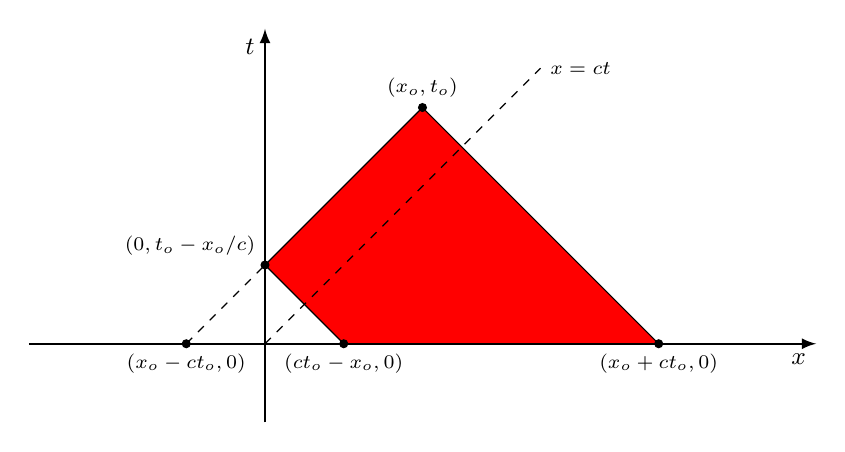
\begin{tikzpicture}
%	\draw[help lines] (-3.5,0) grid (7,5);
	\path [fill=red] (2,3) -- (0,1) -- (1,0) -- (5,0) -- (2,3);
	\draw [->, thick] (-3,0) -- (7,0) node [below left] {\small$x$};
	\draw [->, thick] (0,-1) -- (0,4)  node [below left] {\small$t$};
	\draw [dashed] (-1,0) -- (0,1);
	\draw (0,1) -- (2,3);
	\draw (2,3) -- (5,0);
	\draw [dashed] (0,0) -- (3.5,3.5) node [right] {\scriptsize$x=ct$};
	\draw (0,1) -- (1,0);
	\draw [fill] (2,3) circle [radius=.05] node [above] {\scriptsize$(x_{o},t_{o})$};
	\draw [fill] (5,0) circle [radius=.05] node [below] {\scriptsize$(x_{o}+ct_{o},0)$};	
	\draw [fill] (-1,0) circle [radius=.05] node [below] {\scriptsize$(x_{o}-ct_{o},0)$};
	\draw [fill] (0,1) circle [radius=.05] node [above left] {\scriptsize$(0, t_{o}-x_{o}/c)$};
	\draw [fill] (1,0) circle [radius=.05] node [below] {\scriptsize$(ct_{o}-x_{o},0)$};
\end{tikzpicture}
	
\end{document}